%% ut-thesis.tex -- document template for graduate theses at UofT
%%
%% Copyright (c) 1998-2013 Francois Pitt <fpitt@cs.utoronto.ca>
%% last updated at 16:20 (EDT) on Wed 25 Sep 2013
%%
%% This work may be distributed and/or modified under the conditions of
%% the LaTeX Project Public License, either version 1.3c of this license
%% or (at your option) any later version.
%% The latest version of this license is in
%%     http://www.latex-project.org/lppl.txt
%% and version 1.3c or later is part of all distributions of LaTeX
%% version 2005/12/01 or later.
%%
%% This work has the LPPL maintenance status "maintained".
%%
%% The Current Maintainer of this work is
%% Francois Pitt <fpitt@cs.utoronto.ca>.
%%
%% This work consists of the files listed in the accompanying README.

%% SUMMARY OF FEATURES:
%%
%% All environments, commands, and options provided by the `ut-thesis'
%% class will be described below, at the point where they should appear
%% in the document.  See the file `ut-thesis.cls' for more details.
%%
%% To explicitly set the pagestyle of any blank page inserted with
%% \cleardoublepage, use one of \clearemptydoublepage,
%% \clearplaindoublepage, \clearthesisdoublepage, or
%% \clearstandarddoublepage (to use the style currently in effect).
%%
%% For single-spaced quotes or quotations, use the `longquote' and
%% `longquotation' environments.


%%%%%%%%%%%%         PREAMBLE         %%%%%%%%%%%%

%%  - Default settings format a final copy (single-sided, normal
%%    margins, one-and-a-half-spaced with single-spaced notes).
%%  - For a rough copy (double-sided, normal margins, double-spaced,
%%    with the word "DRAFT" printed at each corner of every page), use
%%    the `draft' option.
%%  - The default global line spacing can be changed with one of the
%%    options `singlespaced', `onehalfspaced', or `doublespaced'.
%%  - Footnotes and marginal notes are all single-spaced by default, but
%%    can be made to have the same spacing as the rest of the document
%%    by using the option `standardspacednotes'.
%%  - The size of the margins can be changed with one of the options:
%%     . `narrowmargins' (1 1/4" left, 3/4" others),
%%     . `normalmargins' (1 1/4" left, 1" others),
%%     . `widemargins' (1 1/4" all),
%%     . `extrawidemargins' (1 1/2" all).
%%  - The pagestyle of "cleared" pages (empty pages inserted in
%%    two-sided documents to put the next page on the right-hand side)
%%    can be set with one of the options `cleardoublepagestyleempty',
%%    `cleardoublepagestyleplain', or `cleardoublepagestylestandard'.
%%  - Any other standard option for the `report' document class can be
%%    used to override the default or draft settings (such as `10pt',
%%    `11pt', `12pt'), and standard LaTeX packages can be used to
%%    further customize the layout and/or formatting of the document.

%% *** Add any desired options. ***
\documentclass{ut-thesis}

%% *** Add \usepackage declarations here. ***
%% The standard packages `geometry' and `setspace' are already loaded by
%% `ut-thesis' -- see their documentation for details of the features
%% they provide.  In particular, you may use the \geometry command here
%% to adjust the margins if none of the ut-thesis options are suitable
%% (see the `geometry' package for details).  You may also use the
%% \setstretch command to set the line spacing to a value other than
%% single, one-and-a-half, or double spaced (see the `setspace' package
%% for details).
\usepackage{graphicx}

%%%%%%%%%%%%%%%%%%%%%%%%%%%%%%%%%%%%%%%%%%%%%%%%%%%%%%%%%%%%%%%%%%%%%%%%
%%                                                                    %%
%%                   ***   I M P O R T A N T   ***                    %%
%%                                                                    %%
%%  Fill in the following fields with the required information:       %%
%%   - \degree{...}       name of the degree obtained                 %%
%%   - \department{...}   name of the graduate department             %%
%%   - \gradyear{...}     year of graduation                          %%
%%   - \author{...}       name of the author                          %%
%%   - \title{...}        title of the thesis                         %%
%%%%%%%%%%%%%%%%%%%%%%%%%%%%%%%%%%%%%%%%%%%%%%%%%%%%%%%%%%%%%%%%%%%%%%%%

%% *** Change this example to appropriate values. ***
\degree{Master of Applied Science}
\department{Civil Engineering}
\gradyear{2019}
\author{Stepan Oskin}
\title{Developing a Python-SQL back-end to join urban data collected from multiple sources.
Design and implementation of a housing market database for Greater Toronto and Hamilton area.
Part of a Longitudinal Analysis of housing sales in the Greater Toronto-Hamilton Area.}


%% *** NOTE ***
%% Put here all other formatting commands that belong in the preamble.
%% In particular, you should put all of your \newcommand's,
%% \newenvironment's, \newtheorem's, etc. (in other words, all the
%% global definitions that you will need throughout your thesis) in a
%% separate file and use "\input{filename}" to input it here.


%% *** Adjust the following settings as desired. ***

%% List only down to subsections in the table of contents;
%% 0=chapter, 1=section, 2=subsection, 3=subsubsection, etc.
\setcounter{tocdepth}{2}

%% Make each page fill up the entire page.
\flushbottom


%%%%%%%%%%%%      MAIN  DOCUMENT      %%%%%%%%%%%%

\begin{document}

%% This sets the page style and numbering for preliminary sections.
\begin{preliminary}

%% This generates the title page from the information given above.
\maketitle

%% There should be NOTHING between the title page and abstract.
%% However, if your document is two-sided and you want the abstract
%% _not_ to appear on the back of the title page, then uncomment the
%% following line.
%\cleardoublepage

%% This generates the abstract page, with the line spacing adjusted
%% according to SGS guidelines.
\begin{abstract}
%% *** Put your Abstract here. ***
%% (At most 150 words for M.Sc. or 350 words for Ph.D.)
    Teranet dataset of real estate transactions recorded in the Province of Ontario holds a wealth of information on the housing market of Ontario, but is very limited in the number of available attributes.
    The dataset can be augmented by joining additional attributes from various data sources, such as Census or TTS survey, based on spatial and/or temporal relationships.
    These relationships are best organized in the form of a relational database based on a database management system, such as PostgreSQL .
    Primary focus of this master's thesis is design and implementation of the proposed GTHA housing market database.
\end{abstract}

%% Anything placed between the abstract and table of contents will
%% appear on a separate page since the abstract ends with \newpage and
%% the table of contents starts with \clearpage.  Use \cleardoublepage
%% for anything that you want to appear on a right-hand page.

%% This generates a "dedication" section, if needed -- just a paragraph
%% formatted flush right (uncomment to have it appear in the document).
%\begin{dedication}
%% *** Put your Dedication here. ***
%\end{dedication}

%% The `dedication' and `acknowledgements' sections do not create new
%% pages so if you want the two sections to appear on separate pages,
%% uncomment the following line.
%\newpage  % separate pages for dedication and acknowledgements

%% Alternatively, if you leave both on the same page, it is probably a
%% good idea to add a bit of extra vertical space in between the two --
%% for example, as follows (adjust as desired).
%\vspace{.5in}  % vertical space between dedication and acknowledgements

%% This generates an "acknowledgements" section, if needed
%% (uncomment to have it appear in the document).
%\begin{acknowledgements}
%% *** Put your Acknowledgements here. ***
%\end{acknowledgements}

%% This generates the Table of Contents (on a separate page).
\tableofcontents

%% This generates the List of Tables (on a separate page), if needed
%% (uncomment to have it appear in the document).
%\listoftables

%% This generates the List of Figures (on a separate page), if needed
%% (uncomment to have it appear in the document).
%\listoffigures

%% You can add commands here to generate any other material that belongs
%% in the head matter (for example, List of Plates, Index of Symbols, or
%% List of Appendices).

%% End of the preliminary sections: reset page style and numbering.
\end{preliminary}


%%%%%%%%%%%%%%%%%%%%%%%%%%%%%%%%%%%%%%%%%%%%%%%%%%%%%%%%%%%%%%%%%%%%%%%%
%%  Put your Chapters here; the easiest way to do this is to keep     %%
%%  each chapter in a separate file and `\include' all the files.     %%
%%  Each chapter file should start with "\chapter{ChapterName}".      %%
%%  Note that using `\include' instead of `\input' will make each     %%
%%  chapter start on a new page, and allow you to format only parts   %%
%%  of your thesis at a time by using `\includeonly'.                 %%
%%%%%%%%%%%%%%%%%%%%%%%%%%%%%%%%%%%%%%%%%%%%%%%%%%%%%%%%%%%%%%%%%%%%%%%%

%% *** Include chapter files here. ***
\chapter[Introduction]{Introduction} \label{ch:introduction}

\section{Introduction} \label{sec:intro}
\chapter[Background information]{Background information} \label{ch:background}

\section{Chapter 2: transportation and land use, land registration in Canada and Teranet} \label{sec:chapter_2_intro}

This chapter discusses the complex interaction of land use and transportation, provides a brief overview of the history of development of land use-transportation (LUT) models, presents some legal and historical background for Teranet's dataset of real estate transactions and finishes with discussing challenges of working with Teranet's data and the proposed solution.

\section{Land Use and Transport (LUT) models} \label{sec:evolution_of_models_of_urban_systems}

\subsection{Complexity of urban systems and "wicked" problems} \label{subsec:complexity_and_wicked_problems}

In her famous 1961 book, Jane Jacobs\cite{Jacobs1961} described a city as "a problem in organized complexity";
since then, many other researchers have remarked that urban systems exhibit complex behaviour\cite{Batty2008, Bettencourt2013}.
Complexity of a system can be defined as a state or quality of being intricate or complicated.
For a system to be complex is not necessarily the same as to be complicated;
complex systems can be simple, i.e.\ governed by a single equation.
Complexity of a system has to do with the intrinsic ability of a system to surprise us with its behaviour;
that the system is hard to understand, despite the mechanics of it being relatively simple.

In 1973, a little over a decade after Jacobs, Rittel and Webber\cite{Rittel1973} presented a path-breaking conceptualization;
this conceptualization characterized urban planning problems as "wicked" problems: problems which cannot be definitively described and for which it makes no sense to talk of "optimal solutions".
In their paper, Rittel and Webber stated that such "wicked" problems are never "solved", and that the focus instead becomes on iteratively "re-solving" the problems over and over.
More than 40 years after their original publication, Rittel and Webber's ideas remain relevant to the policy sciences today: there is an intense interest in the nature of "wicked" problems and the complex tasks of identifying their scope, viable responses, and appropriate mechanisms and pathways to improvement\cite{Crowley2017}.
Interaction between land use and transportation, which is discussed in the following section, presents a prime example of urban complexities and "wicked" problems.

\subsection{Transportation-land use cycle} \label{subsec:transportation_land_use_cycle}

Among the reasons why transportation and land use interaction is "wicked" are such aspects as pluralism of expectations among stakeholders, institutional complexity in policy making, and scientific uncertainty\cite{Noto2015}.
More importantly, there is a fundamental link between transportation and urban form: urban form has an enormous impact on the type and cost of transportation systems needed to serve residents of a metropolitan area\cite{Kelly1994}.
Transportation, in turn, influences land development and location choices of people and firms, and thus completes the formation of a feedback relationship that Stover and Koepke\cite{Stover1988} referred to as a cycle.
Interconnections between points (activities) in space can be perceived through the medium of the transportation system\cite{Miller1998}

Figure~\ref{fig:idealized_integrated_urban_model} illustrates the complex interactions between land use and transportation system as summarized by Miller, Kriger and Hunt\cite{Miller1998}.

\begin{figure}[hbt!]
    \centering
    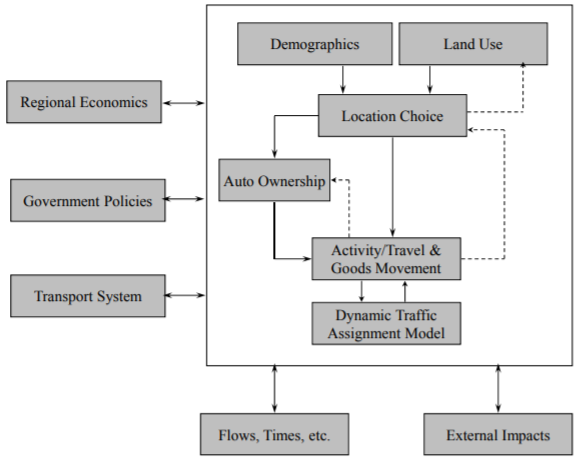
\includegraphics[width=0.7\linewidth,trim=0 0 0 0,clip]{miller_idealized_urban_model.png}
    \caption{An Idealized Integrated Urban Model System, adapted from Miller, Kriger and Hunt\cite{Miller1998}.}
    \label{fig:idealized_integrated_urban_model}
\end{figure}

Many different types of models are used in planning, such as demand forecasting models projecting traffic or ridership, or land use models projecting and distributing population and jobs within an area.
At an earlier stage of model development, some analysts argued that there is no significant link between transportation and land use, given the near-ubiquity of the transportation (road) network\cite{Miller1998}.
However, the unprecedented urban growth of the 21st century introduced new challenges for urban systems such as extreme road congestion, equity of access to jobs and services among low-income households, energy scarcity, environmental and GHG impacts from transportation systems and public health impacts of land use patterns\cite{Miller2018b,Moeckel2017}.

It became apparent that these "transport problems" cannot be solved through transportation policies and investment alone, that the physical design of the city at the "macro" and "micro" scale critically interfaces with the demand for and performance of the transportation system.
In addition, to accurately assess the costs and benefits of an expensive long-term transportation infrastructure investment, "feedback" effects of these investments on urban form, land values, property taxes, quality of life, etc.
need to be quantified and included in evaluation and decision making.
Thus, today there is a steadily growing recognition within the urban policy field that the interaction between transportation and land use does exist and does matter\cite{Miller2018b}.

%TODO change the end of 1st sentence
In the context of models, integrated urban models (IUMs) aim to capture the complex relationship between urban systems such as transportation and land use more accurately.
Integrated land use-transportation models combine travel demand forecasting and land use forecasting functions and recognize that the distribution of population and jobs depends, in part, on transportation accessibility.
The reverse is also true, and thus integrated models incorporate feedback relationship between transportation and land use, with economic decisions by households and firms acting as one of the links between the two systems\cite{Miller1998}.

\subsection{Evolution of LUT models} \label{subsec:evolution_of_lut_models}

The history of treating cities as systems via simulation models of transportation and land use dates back to 1950s when General System Theory and Cybernetics came to be applied in the softer social sciences\cite{Batty2008}.
The first operational simulation model that truly integrated land use and transportation is considered to be A Model of Metropolis built in 1964 by Ira S. Lowry for the Pittsburgh region based on economic base theory\cite{Lowry1964}.
It was a highly aggregate model based on theories of spatial interaction, such as the gravity model that was popular in quantitative geography and transportation planning at the time\cite{Bouchard1965}.
Models based on spatial interaction framework continued to be developed through mid-1980s, until developments in random utility theory allowed researchers to describe choices among discrete alternatives, such as the choice of travel mode, and generate models based on the study of disaggregate behaviour\cite{Iacono2008}.

Figure~\ref{fig:lut_model_evolution} provides the general overview of chronological development of LUT models summarized by Iacono\cite{Iacono2008}.

\begin{figure}[hbt!]
    \centering
    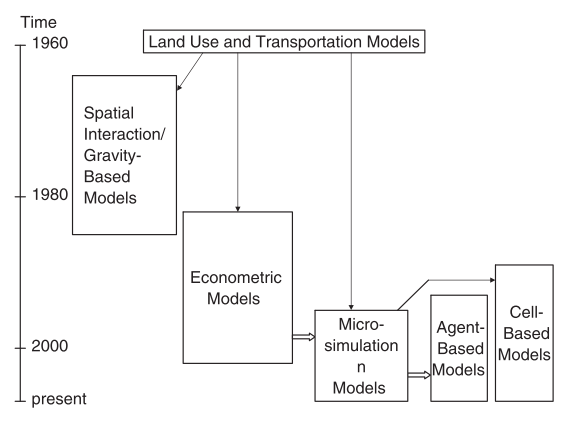
\includegraphics[width=0.7\linewidth,trim=0 0 0 0,clip]{lut_models_evolution.png}
    \caption{Chronological development of LUT models summarized by Iacono\cite{Iacono2008}.}
    \label{fig:lut_model_evolution}
\end{figure}

The modeling paradigm has changed fundamentally in the early 1990s along with the advances in computing power and efficiency of data storage.
Urban systems used to be viewed as hierarchical and centrally organized equilibrium structures, or "top-down".
Instead, now they were considered to be structured from the "bottom-up", dynamically retaining their integrity through interactions of numerous microelements\cite{Batty2008}.
A new broad class of LUT models that could fall under the title of "microsimulation" began to be developed.
It included such classes of models as activity-based travel, cell-based models, and multi-agent models, and more recently comprehensive urban microsimulation models that fully reflect the dynamics of changes in the population and the urban environment\cite{Iacono2008}.
%TODO check last sentence

"Micro" in the microsimulation implies that the model must be highly disaggregated spatially, socio-economically and in its representation of processes.
"Simulation" implies that the model must be numerical, stochastic, have an explicit time dimension, and "evolve" into the end state rather than "solve for it"\cite{Miller2018c}.
An example of such model has been developed by the University of Toronto ILUTE team;
their product is an integrated urban model capable of microsimulating urban demographic evolution, housing markets and travel behaviour over extended periods of time\cite{Miller2018a}.
The ILUTE system and some of the ways for its future improvement are discussed in the following section.

\subsection{ILUTE and HoMES model systems} \label{subsec:ilute}

The Integrated Land Use, Transportation, Environment (ILUTE) model system is an agent-based microsimulation model for greater Toronto-Hamilton area;
it includes such components as land use, activity/travel, urban economics, auto ownership, demographics and emissions/energy use.
It uses disaggregate models of spatial socioeconomic processes to evolve the state of the greater Toronto\textendash Hamilton area from a known base case to a predicted end state in 1-year time steps.
The system state is defined in terms of the individual persons, households, dwelling units, firms, etc.
that collectively define the urban region being modeled\cite{Miller2011}.

ILUTE model simulates the evolution of an urban region's spatial form, demographics, travel behavior and economic structure over time.
Many markets are of interest within ILUTE, such as housing, labour, commercial, real estate, etc.) and are modeled via microsimulation.
The model aims to capture the dynamics of these markets through disaggregated representations.
For example, in the housing market component of ILUTE, houses are auctioned off one dwelling at a time to interested bidders in a disaggregate implementation of Martinez' Bid Choice theory\cite{Martinez1992}.

The Housing Market Evolutionary System (HoMES) is the updated housing market module for the ILUTE model system.
HoMES is a disaggregate, agent-based microsimulation of the owner-occupied housing market that evolves the residential location of households over time and includes the endogenous supply of housing by type and location, as well as the endogenous determination of sales prices and rents.

An overview of the framework of housing market supply, demand and clearing mechanisms utilized in HoMES provided by Rosenfield et al.\cite{Rosenfield2013} is presented on figure~\ref{fig:homes_framework}

\begin{figure}[hbt!]
    \centering
    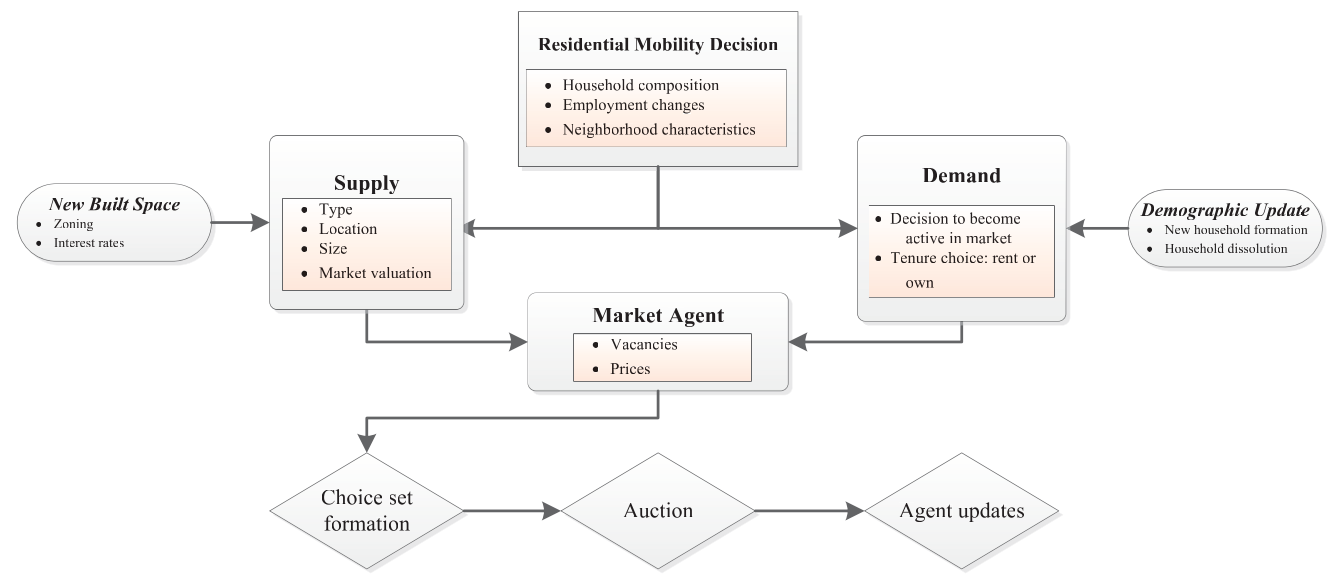
\includegraphics[width=0.99\linewidth,trim=0 0 0 0,clip]{homes_framework.png}
    \caption{Framework of housing market supply, demand and clearing mechanisms used in HoMES module of ILUTE, as summarized by Rosenfield et al.\cite{Rosenfield2013}.}
    \label{fig:homes_framework}
\end{figure}

Among the major barriers to implementation of integrated urban models since their introduction were such aspects as data hungriness and computational requirements\cite{Miller1998}.
However, continuing methodological advances, such as cost-effective High Performance Computing (HPC), detailed GIS-based datasets and machine learning methods, mean that former barriers now represent opportunities for model system development.
In the case of ILUTE and HoMES, one of the possibilities for further improvement is the use of new data sources to update the housing market model.
One of these new data sources, Teranet's dataset of land registry records, and main challenges of working with it are discussed in section~\ref{sec:new_data_sources_and_their_challgenges}.

\section{New data sources and their challenges} \label{sec:new_data_sources_and_their_challgenges}

\subsection{Further improvement of integrated urban models} \label{subsec:further_improvement_of_iums}


As an increasing amount of aspects of human life becomes digitalized, a wealth of new data is produced and can be used to model and analyze dynamics of urban systems\cite{Arribas-Bel2014, Chen2016}.
An example of such digitalization of human activity is the introduction of the Province of Ontario Land Registration Information System (POLARIS) in 1985 by the Government of Ontario\cite{TeranetEnterprisesInc.} that will be discussed in the following section.
Introduction of POLARIS lead to the creation of an extensive dataset of real estate transactions (land registration records) by the Teranet Enterprises Inc.
This dataset offers a very fine resolution of housing market dynamics across both time and space, which can be beneficial for updating and testing microsimulation models, but it also presents challenges to work with that will be discussed in section~\ref{subsec:teranet_ontario} of this chapter;
the chapter concludes with the proposed solution to address one of the main challenges of working with Teranet's data.

\subsection{POLARIS: electronic system of land registration in Ontario} \label{subsec:land_reg_system_canada}

All land owned in Canada is registered in a public land registry in the applicable province.
Each province and territory in Canada has its own land registry system, whether it is a land titles system, a registry system or a combination of both, with each system having its own rules.
The registry system is a public record of documents evidencing transactions affecting land.
In the land titles system, the applicable provincial government determines the quality of the title, and essentially guarantees (within certain statutory limits) the title to, and interests in, the property.
As of 2015, most common law provinces and territories in Canada were using the land titles system or were in the process of converting from a registry system to a land titles system\cite{McKean2015}.

As of 2015, the Province of Ontario has largely converted from registry systems to a land titles system.
In 1985, the Government of Ontario initiated the Province of Ontario Land Registration Information System (POLARIS) pilot project for the purposes of the conversion between systems and records automation.
The Land Registration Reform Act (Ontario)\cite{TheGovernmentofOntario1990} was introduced in 1990 to facilitate electronic search and registration of properties and the automation of paper-based records.
POLARIS was built by the Province to house and process electronic land records, which in turn lead to the creation of an extensive dataset of land registration records managed by Teranet Enterprises Inc.
Today, POLARIS is the search/registration and property maintenance system for all automated land records in Ontario.

\subsection{The Teranet-Ontario Partnership, Teranet's data and its challenges} \label{subsec:teranet_ontario}

In 1991, the Government of Ontario established a partnership with Teranet, a Toronto-based organization, founded the same year, which provides e-services to legal, real estate, government, financial, and healthcare markets.
The partnership was established to convert Ontario's land registration system to a more modernized electronic title system.
The project involved taking a 200-year-old paper-based system and creating a database with electronic records for more than five million parcels of land.
Teranet converted all qualified Registry properties in Ontario to the Land Titles system and automated existing paper Land Titles parcels.
As a result, 99.9\% of property in Ontario was parcelized and administered under the Land Titles system.
Teranet fully automated the conversion of millions of paper-based documents and records into the Ontario Electronic Land Registration System (ELRS)\cite{TeranetEnterprisesInc.2019}.


Teranet dataset presents an extensive historical record of real estate transactions recorded in the Province of Ontario since the beginning of XIX century.
However, when it comes to using new data sources in social studies, along with opportunities there are also challenges present.
For example, these data sources can have issues with the quality of the data, might require a specific set of skills to take advantage of these data sources, or might not be suitable for traditional methods meant for traditional data\cite{Arribas-Bel2014}, all of which are true in the case of Teranet's dataset.

One of the major attributes missing from the available version of Teranet's dataset is the information about the type of property being transacted, with records of various residential, commercial and industrial properties all being mixed together in the same dataset.
At the same time, Teranet records have timestamps (dates) and location information (x and y coordinates) and thus can be joined to variety of other urban data sources, such as Census demographics, Transportation Tomorrow Survey (TTS) and parcel-level land use information.
It is possible to derive this attribute from additional related sources of information, such as detailed land use or Census demographics.
However, joining these data sources together requires additional considerations, as they use different spatial units and are available at different temporal spans, as will be discussed in chapter~\ref{ch:spatial_and_temporal_relationships_between_urban_data}.


\section{Chapter summary} \label{sec:background_summary}

The fundamental link between transportation and urban form creates a feedback relationship between land development, travel needs, viability of alternative modes, accessibility, and other important characteristics of the urban transportation system.
Numerous "top-down" and "bottom-up" models have been designed to analyze and forecast the behaviour of urban regions and interaction of their transportation and land use systems.
Since urban systems are complex in nature and require "re-solving" over and over, data science process models present a good fit for this task with their iterative structure.

Increased digitization of human activity, such as introduction of POLARIS land registration system by the Government of Ontario in 1985, produce a wealth of new information that can be used to study interaction between land use and transportation at a fine spatial and temporal scale.
Teranet's dataset of real estate transactions presents a wealth of information on the housing market of Ontario and can be used for empirical studies of transportation-land use interaction.
However, along with the opportunities, the new data sources also present new challenges.
Teranet's dataset has some data quality issues that need to be addressed and might require special skills to work with due to its size.
But most importantly, it is very limited in the number of features available for each transaction.

One of the major attributes missing from the available version of Teranet's dataset is the information about the type of property being transacted, with records of various residential, commercial and industrial properties all being mixed together in the same dataset.
At the same time, Teranet records have timestamps (dates) and location information (x and y coordinates) and thus can be joined to variety of other urban data sources, such as Census demographics, Transportation Tomorrow Survey (TTS) and parcel-level land use information.
It is possible to derive this attribute from additional related sources of information, such as detailed land use or Census demographics.
However, joining these data sources together requires additional considerations, as they use different spatial units and are available at different temporal spans, as will be discussed in chapter~\ref{ch:spatial_and_temporal_relationships_between_urban_data}.

\chapter{Spatial and temporal relationships between data sources} \label{ch:spatial_and_temporal_relationships}

The second phase of CRISP-DM process model for data mining projects is data understanding;
this chapter discusses the nature of spatial and temporal relationships of different data sources that are used in this master's thesis.
As was discussed in section~\ref{sec:teranet_challenges_solution}, one of the main challenges of working with Teranet's data is the lack of available features.
At the same time, Teranet records have timestamps (dates) and location information (x and y coordinates) and thus can be joined to a variety of other urban data sources, such as Census demographics, Transportation Tomorrow Survey (TTS) and parcel-level land use information.
However, as will be discussed in this chapter, these data sources use different spatial units and are available at different temporal spans;
therefore, special consideration must be taken when joining data from these sources with respect to their temporal and spatial relationships to ensure semantic interoperability.

Different data sources joined to Teranet's dataset are described in this chapter, the implementation of the spatial and temporal relationships via the standardized data preparation workflow in Python and a PostgreSQL relational database are described in chapter~\ref{ch:data_preparation}.

\section{Description of data sources used} \label{sec:description_of_data_sources}

The following data sources were combined into the GTHA housing market database that was created as a part of this master's thesis:

\begin{enumerate}
    \item Teranet's dataset

    Due to the introduction of POLARIS by the Province of Ontario in 1985 (discussed in section~\ref{sec:polaris}), Teranet's dataset includes a complete population of real estate transactions recorded in Ontario from 1985 up to October of 2017 (records prior to 1985 appear to be incomplete, see figure~\ref{fig:teranet_time_series}).
    Since Teranet's dataset has a high number of records, it can be used to investigate aspects relating to the housing market at a very fine spatial and temporal scale.


    \begin{figure}[hbt!]
        \centering
        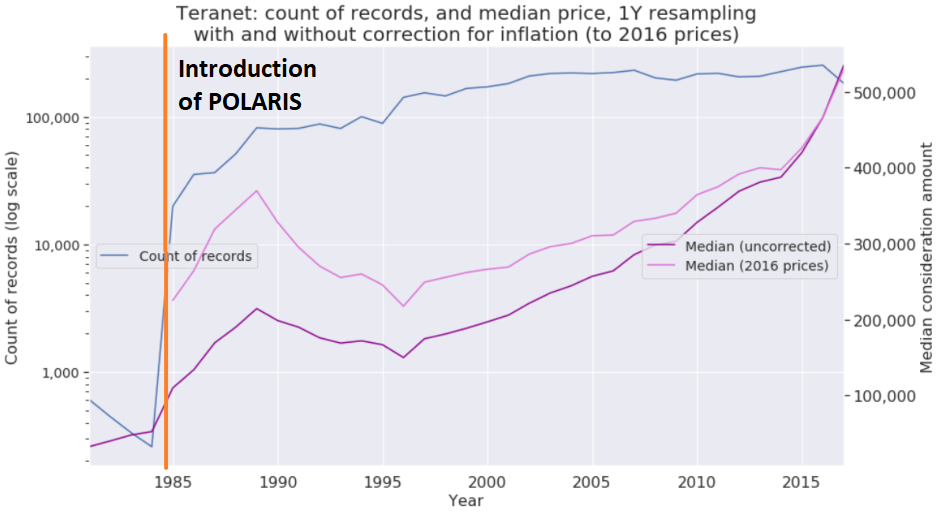
\includegraphics[width=1\linewidth,trim=0 0 0 0,clip]{teranet_time_series.png}
        \caption{Time series of total count of Teranet records within GTHA boundary (log scale, left y-axis) and their median consideration amount (right y-axis), resampled by 1-year intervals.
        It can be seen that there is a dramatic increase in the total count of records between 1984 and 1985, which coincides with the introduction of POLARIS electronic land registration system by the Government of Ontarion in 1985, which was discussed in section~\ref{sec:polaris}.
        Teranet records prior to 1985 appear to be incomplete.}
        \label{fig:teranet_time_series}
    \end{figure}

    \item Select variables from the Census of Canada

    One of the major sources of demographic and statistical data in Canada are the datasets collected under the national Census program.
    Census datasets provide valuable insights into the latest economic, social and demographic conditions and trends in Canada and are used to plan important public services.
    Statistics Canada collects every five years the national Census of Canada and disseminates the information by a range of geographic units, also referred to as "Census geography"\cite{MapandDataLibrary2019}.

    \item Select variables from the Transportation Tomorrow Survey (TTS)

    Another major source of information for most transportation planning studies concerned with Southern Ontario is the Transportation Tomorrow Survey (TTS), an origin-destination travel survey\cite{DataManagementGroup2014}.
    The Transportation Tomorrow Survey (TTS), undertaken every five years since 1986, is a cooperative effort by local and provincial government agencies to collect information about urban travel in southern Ontario.
    TTS represents a retrospective survey of travel taken by every member (age 11 or over) of the household during the day previous to the telephone or web contact.
    The information collected and the method of collection has remained relatively consistent over the seven surveys;
    TTS survey data includes characteristics of the household, characteristics of each person in the household, and details of the trips taken by each member of the household, including details on any trips taken by transit\cite{Ashby2018}.

    \item Land use from DMTI Spatial Inc.\ by year (2001-2014)

    DMTI Spatial Inc., a Digital Map Products company, is a major provider of location based information in Canada.
    DMTI has been providing industry leading enterprise Location Intelligence solutions for more than a decade to Global 2000 companies and government agencies\cite{DMTISpatialInc.2014}.

    \item Detailed land use information from University of Toronto's Department of Geography collected in 2012 and 2013

    The detailed land-use data provided by University of Toronto's Department of Geography is a combination of parcel boundaries (from Teranet) and manually coded land-use data produced using Google maps and streetviews;
    it was collected by Prof.\ Andre Sorensen and Prof.\ Paul Hess's research project.

\end{enumerate}

\section{Spatial relationships between data sources} \label{sec:spatial_relationships}

Most urban areas are divided into zones or planning areas on the basis of maintaining similar population sizes and following built or natural boundaries like roads or rivers.
Census geography follows a certain hierarchy defined by Statistics Canada, with the largest top-level divisions being provinces and territories, and the lowest-tier divisions to which Census data is disseminated being Dissemination Areas (DAs)\cite{StatisticsCanada2018}.
Statistics Canada defines a Dissemination Area as a small area composed of one or more neighbouring dissemination blocks, roughly uniform in population size targeted from 400 to 700 persons to avoid data suppression\cite{StatisticsCanada2015}.

To simulate the changes in accessibility, metropolitan regions are usually broken down into a set of small geographic zones, similar (or in many cases identical) to the set of zones used for regional travel forecasting.
For TTS variables, the finest level of spatial aggregation is that of the Traffic Zone, also referred to as the Traffic Analysis Zone (TAZ).
A Traffic Zone is a polygon which typically falls along the centre line of roads or the natural geographic boundaries\cite{DataManagementGroup2019}.
Not as a rule, but TAZ zones roughly follow Census tract boundaries, which are slightly bigger than DA boundaries.
Figure~\ref{fig:da_taz_difference} presents an example of TAZ polygons overlaid with Census DA boundaries.

\begin{figure}[hbt!]
    \centering
    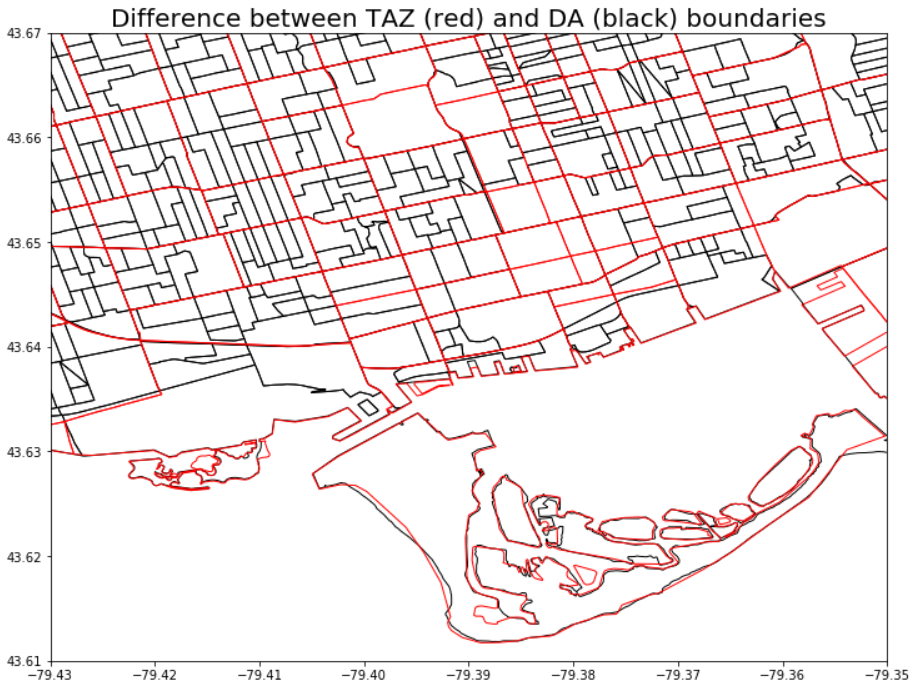
\includegraphics[width=0.7\linewidth,trim=0 0 0 0,clip]{da_taz_difference.png}
    \caption{Spatial relationship between datasets: difference between Traffic Analysis Zones (TAZ, red) and Census Dissemination Area (DA, black).}
    \label{fig:da_taz_difference}
\end{figure}

TTS data has been collected for changing TAZ boundaries, or in other words, different zone systems due to growing population and expanding extents of the survey in the GTHA region over the years.
To make the TTS data consistent for comparing over all years from 1986 to 2016, the Data Management Group (DMG) at the University of Toronto Transportation Research Institute (UTTRI), the custodian of the dataset derived from TTS, made all surveys available in the 2001 zone system, for convenience of researchers (any zone system could have been chosen for that matter).
UTTRI used the 2001 TAZ system to model travel times for the GTHA on EMME for all TTS years based on the origin-destination trip data collected in the survey.
The travel time data was used to create further transportation accessibility variables.

Land use data collected by DMTI and by the Department of Geography uses the spatial unit of a parcel polygon.
Teranet records have attributes representing x and y coordinates matching parcel centroids.

\vspace{5mm}

Below is the summary of spatial units used by the data sources that were combined into the GTHA housing market database, designed and implemented as a part of this master's thesis:

\begin{itemize}
    \item Point data
    \begin{itemize}
        \item Teranet
    \end{itemize}
    \item Parcel-level data (polygons)
    \begin{itemize}
        \item detailed land use from the Department of Geography
        \item land use from DMTI
    \end{itemize}
    \item DA-level data (polygons)
    \begin{itemize}
        \item Census variables
    \end{itemize}
    \item TAZ-level data
    \begin{itemize}
        \item TTS variables
    \end{itemize}
\end{itemize}

When joining these data sources, difference in spatial units needs to be respected, which can be more challenging when spatially joining polygons with polygons, since it might require area-weighted spatial interpolation of data to a common unit of analysis.
In addition, polygon-based data can also vary with time, as is the case with DMTI's land use information, which is available by year.
To simplify relating different polygon-based data sources with each other, all of them can be brought together to a single level of time-indexed points, such as Teranet transactions.
This allows flexibility in combining data from polygon-based data sources to a common point level while maintaining the integrity of spatial and temporal relationships through polygon-to-point spatial joins.
Implementation of these relationships is described in chapter~\ref{ch:data_preparation}, temporal relationships between different data sources are described in the following section.

\section{Temporal relationships between data sources} \label{sec:termporal_relationships_between_datasets}

In addition to using different spatial units, data sources joined with Teranet's dataset are available at different temporal spans:
\begin{itemize}
    \item Teranet records have individual timestamps (date) on each record
    \item Census and TTS variables are sampled once in 5 years
    \item DMTI's land use data is available by year and covers a time span from 2001 to 2014
    \item Detailed land use from the Department of Geography was collected at a single point in time during the summers of 2012 and 2013
\end{itemize}

Temporal matching between Teranet records and DMTI data can be done directly: DMTI land use for each year from 2001 to 2014 can be spatially joined with a subset of Teranet records from the corresponding year;
such approach would ignore changes of land use types that occur within a year, but would recognize land use changes between the years for which DMTI land use data is available.
Since the detailed land use provided by the Department of Geography was collected at a single point in time, it can be joined to all Teranet records;
however, it should be kept in mind that this land use data will be the most accurate around its time of collection in 2012 and 2013, and will become increasingly less accurate with an increase of the temporal span of Teranet records.

\begin{figure}[hbt!]
    \centering
    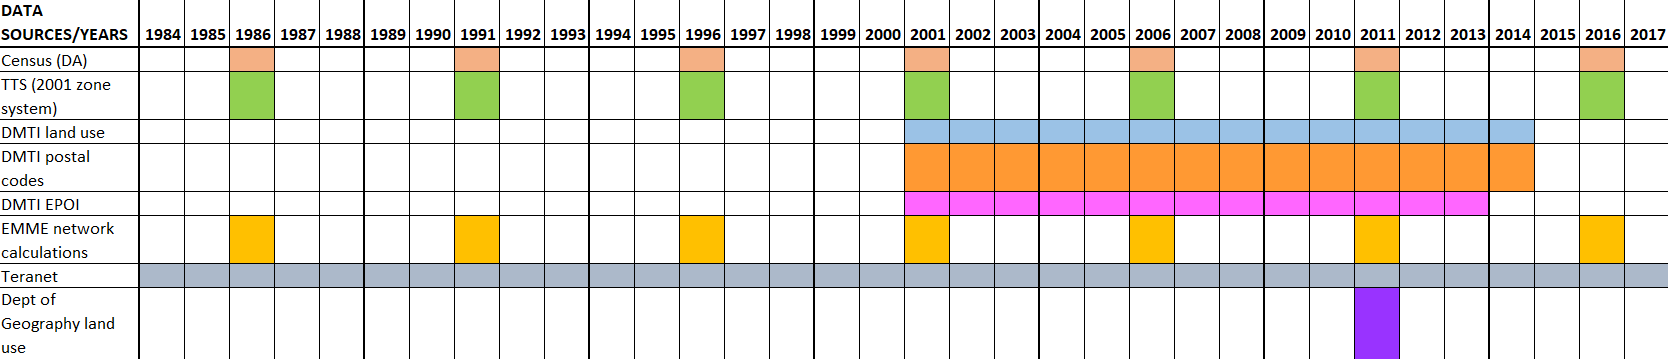
\includegraphics[width=1\linewidth,trim=0 0 0 0,clip]{temporal_spans.png}
    \caption{Temporal spans of data sources used in the GTHA housing market database.}
    \label{fig:temporal_spans}
\end{figure}

\vspace{5mm}

As for Teranet and Census / TTS variables, they can be matched in a number of ways:

\begin{enumerate}
    \item Direct match with appropriate Teranet subsets
    \begin{itemize}
        \item match Census / TTS variables only with Teranet records from the corresponding year (for example, Teranet records from 2016 matched with 2016 Census / TTS variables)
        \item benefits:
        \begin{itemize}
            \item Census / TTS variables would be composed of the actual values recorded by the survey
        \end{itemize}
        \item disadvantages:
        \begin{itemize}
            \item limited use of Teranet data since only records from Census / TTS years can be matched
        \end{itemize}
    \end{itemize}
    \item Interpolation of discrete Census / TTS variables
    \begin{itemize}
        \item discrete Census / TTS variables can be turned into continuous via interpolation
        \item benefits:
        \begin{itemize}
            \item closest temporal match between Teranet and Census / TTS variables
        \end{itemize}
        \item disadvantages:
        \begin{itemize}
            \item additional assumptions need to be made for each Census / TTS variable
        \end{itemize}
    \end{itemize}
    \item Assign temporal spans to each Census / TTS survey as new features to Teranet records
    \begin{itemize}
        \item each Census / TTS survey is assigned a temporal span of 5 years;
        this 5-year span represents a group of Teranet records to which variables from this survey can be matched (for example, Census variables of 2016 are matched with Teranet record from 2014 to 2018)
        \item benefits:
        \begin{itemize}
            \item avoid interpolation assumptions
        \end{itemize}
        \item disadvantages:
        \begin{itemize}
            \item step-change in Census / TTS variables
        \end{itemize}
    \end{itemize}
\end{enumerate}

To avoid additional interpolation assumptions and use the actual values recorded from Census and TTS surveys, the third option has been chosen for matching Teranet records with Census / TTS variables.
Each Census / TTS survey is assigned a 5-year time span centered at the survey year (i.e., 2014--2018 for 2016 survey year) and new foreign keys are introduced to Teranet records to allow matching with 5-year time spans of Census / TTS variables.
Implementation of temporal relationships for Teranet records will be described in chapter~\ref{ch:data_preparation}.
Figure~\ref{fig:temporal_spans} presents the temporal spans assigned to each data source for joining with Teranet records.

\section{Chapter summary} \label{sec:data_sources_summary}

Variables that can be joined to augment Teranet's dataset, such as Census and TTS surveys and parcel-level land use data, are defined using different spatial units and are available at varying temporal spans.
These relationships need to be respected when combining variables from these data sources into a single dataset to ensure semantic interoperability.
The integrity of spatial relationships can be ensured by spatially joining all polygon-based data sources to Teranet points.
Temporal relationships between DMTI land use and Teranet sales records are incorporated by performing separate spatial join operations for each annual DMTI land use dataset with a corresponding Teranet subset.
For Census and TTS variables, additional foreign keys are introduced assigning 5-year spans to each Teranet record corresponding to a Census / TTS survey;
these foreign keys indicate which Teranet records should be joined to a particular Census or TTS survey.
Implementation of these relationships via a standardized data preparation workflow in Python and a PostgreSQL relational database are described in chapter~\ref{ch:data_preparation}.

\chapter{Data preparation} \label{ch:data_preparation}

The "wicked" nature of transportation and land use interaction introduced in chapter~\ref{ch:background} dictates the need to iteratively "re-solve" transportation and land use planning problems instead of focusing on finding some single "optimal solution".
This approach resembles the methodologies typically employed for data science projects, where the sequence of steps is iterated over, producing a more meaningful solution on each new iteration of the cycle, as defined by such process models as CRISP-DM\cite{Shearer2000}.
Similarly, data preparation can be followed in a linear manner, but is very likely to be iterative in nature\cite{Brownlee2013}.

\vspace{5mm}

Data preparation plays a critical role in research projects:

\begin{itemize}
    \item it can determine the success of applications of machine learning algorithms
    \item it is a prerequisite for any meaningful analysis
    \item it is often required to allow the introduction of constraints necessary for implementation of RDBMS
\end{itemize}

\vspace{5mm}

To facilitate easy modification and replication of the data preparation process for data sources related to the GTHA housing market, a streamlined data preparation workflow using Python via a series of jupyter notebooks has been established as a part of this master's thesis.
It accomplishes three main objectives:
\begin{itemize}
    \item clean Teranet dataset and correct its records for consistency
    \item introduce new keys that allow efficient joining of other data sources such as Census or TTS, while maintaining the integrity of spatial and temporal relationships that were discussed in chapter~\ref{ch:spatial_and_temporal_relationships}
    \item engineer new features that can be used by the machine learning algorithm along with the features from the joined datasets to classify land use, which will be discussed in chapter~\ref{ch:ml_workflow}
\end{itemize}

This chapter introduces the concepts of ''Tidy Data'' and database normalization and outlines the standardized data preparation workflow for all data sources related to the GTHA housing market.

\section{Tidy data and database normalization} \label{sec:db_norm_tidy_data}

Hadley Wickham in his paper ''Tidy Data''\cite{Wickham2014} formalized the way how a shape of the data can be described and what goal should be pursued when formatting data.
The tidy data standard is closely related to Edgar F. Codd's relational algebra and has been designed to facilitate initial exploration and analysis of the data, and to simplify the development of data analysis tools that work well together.
As an integral part of his relational model, Codd\cite{Codd1990} proposed a process of database normalization, or restructuring of a relational database in accordance with a series of so-called normal forms in order to reduce data redundancy and improve data integrity.
Normalization entails organizing the columns (attributes) and tables (relations) of a database to ensure that their dependencies are properly enforced by database integrity constraints.
The principles of ''tidy data'' essentially reformulate Codd's ideas in statistical language.

According to Wickham\cite{Wickham2014}, ''tidy data'' is a standard way of mapping the meaning of a dataset to its structure.
A dataset is ''messy'' or ''tidy'' depending on how rows, columns and tables are matched up with observations, variables and types.

\vspace{5mm}

In ''tidy data'':
\begin{enumerate}
    \item Each variable forms a column.
    \item Each observation forms a row.
    \item Each type of observational unit forms a table.
\end{enumerate}

This is Codd's 3rd normal form\cite{Codd1990}, but with the constraints framed in statistical language, and the focus put on a single dataset rather than the many connected datasets common in relational databases.
''Messy data'' is any other arrangement of the data.

\vspace{5mm}

The structure of Teranet's dataset conforms with the ''Tidy data'' format.
Contrary to Teranet, tables with combined selected Census and TTS variables have variables for different Census and TTS years recorded as columns.
This needs to be addressed by ''melting'' these tables and introducing a new attribute 'year' to be used as a part of a composite foreign key when joining with Teranet records.

\vspace{5mm}

Census and TTS tables were ''melted'' into the ''tidy data'' format:
\begin{itemize}
    \item each Census / TTS variable now forms a single column
    \item each value of a variable is indexed by a composite primary key constituting of spatial identifier and year of the survey
    \item spatial identifiers are 'DAUID' or 'TAZ\_O' (unique identifier for Dissemination Areas or Traffic Analysis Zones introduced in section~\ref{sec:spatial_relationships})
\end{itemize}

Introduction of new foreign keys is described in the following section.

\section{Introduction of new keys and attributes via spatial and temporal relationships} \label{sec:introduction_of_new_keys}

As no combination of columns constitutes a candidate key for Teranet records (unique identifier to be used in RDBMS), a surrogate key (artificial unique identifier for RDBMS) is added to the Teranet dataset via a new attribute 'transaction\_id'.
Thus, Teranet's dataset fits into a normalized database, with the new attribute 'transaction\_id' as its primary key.
As was discussed in section~\ref{sec:db_norm_tidy_data}, the ''melted'' Census and TTS tables have composite primary keys consisting of a unique spatial identifier ('DAUID' or 'TAZ\_O', respectively) and the year of the survey.

To implement the spatial and temporal relationships between the data sources discussed in chapter~\ref{ch:spatial_and_temporal_relationships}, a number of new foreign keys needed to be introduced to Teranet records.
The new foreign keys either represent spatial identifiers (such as 'dauid' or 'taz\_o', corresponding to DA or TAZ within which a Teranet record is located), or an attribute identifying the year of the Census or TTS survey to which this Teranet record can be joined.
Foreign keys representing spatial identifiers are added through a series of spatial joins while foreign keys identifying temporal spans are produced based on temporal relationships established in section~\ref{sec:termporal_relationships_between_datasets}.

\vspace{5mm}

New spatial identifiers were introduced to each Teranet record via a series of spatial joins:
\begin{enumerate}
    \item 9'039'241 Teranet points were joined with 9'182 polygons of Dissemination Areas (DAs) for GTHA used by Census variables
    \begin{itemize}
        \item Teranet records with coordinates falling outside of GTHA boundary were filtered out
        \item From the original 9'039'241 records, 6'803'691 remained in the dataset
        \item New foreign keys 'dauid', 'csduid' and attribute 'csdname' were added to each Teranet record
    \end{itemize}
    \item 6,803,691 Teranet points were joined with 1,716 polygons of Traffic Analysis Zones (TAZ) used by TTS variables
    \begin{itemize}
        \item New foreign key 'taz\_o' was added to each Teranet record
    \end{itemize}
    \item 6,803,691 Teranet points were joined with 525 polygons of Forward Sortation Areas (FSA) and 555,668 polygons of postal geography from DMTI's Platinum Postal Geography Suite
    \begin{itemize}
        \item New foreign keys 'fsa' and 'pca\_id' and attribute 'postal\_code\_dmti' were added to each Teranet record
        \item These keys are not currently used for joining any variables, but were added to expand the potential for relating datasets
    \end{itemize}
    \item 6,803,691 Teranet points were joined with 1,664,862 polygons of parcel-level detailed land use provided by the Department of Geography
    \begin{itemize}
        \item New foreign keys 'pin\_lu', 'landuse' and 'prop\_code' were added to each Teranet record
        \item Foreign keys 'landuse' and 'prop\_code' are codes that can be converted to land use categories that were used by the Department of Geography for GTA and Hamilton, respectively
        \item For records from Hamilton, 'prop\_code' was converted to categories used by GTA land use and reassigned to 'landuse', bringing GTA and Hamilton records to a single system of land use categories
    \end{itemize}
    \item Subsets of Teranet points were joined with corresponding yearly polygons of parcel-level land use from DMTI
    \begin{itemize}
        \item New attribute 'dmti\_lu' was added to each Teranet record
    \end{itemize}
\end{enumerate}

\begin{figure}[hbt!]
    \centering
    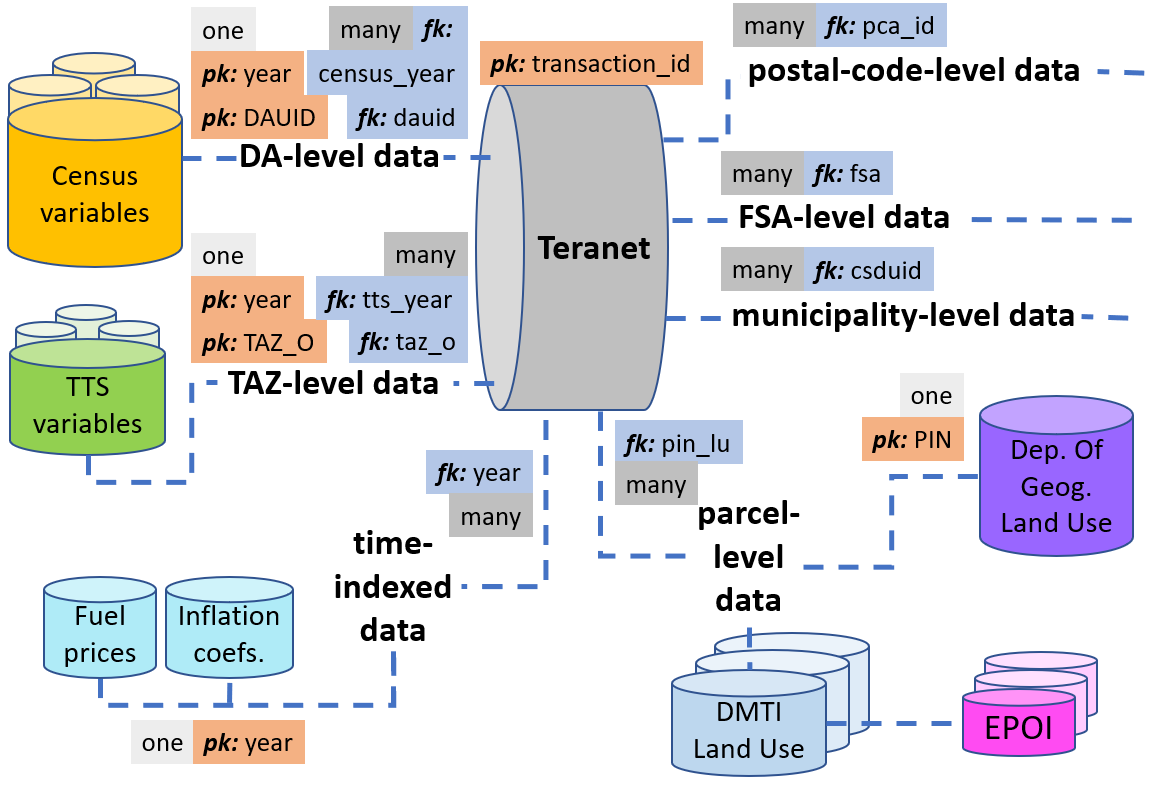
\includegraphics[width=1\linewidth,trim=0 0 0 0,clip]{data_relations.png}
    \caption{Relationships between datasets introduced during data preparation were then used to set up referential integrity constraints of the new PostgreSQL database for GTHA housing market data.}
    \label{fig:data_relations}
\end{figure}

Foreign keys representing temporal identifiers are generated from the registration date of each Teranet record, matching each year of Teranet records to a corresponding 5-year span covered by a Census or TTS survey, as was discussed in section~\ref{sec:termporal_relationships_between_datasets}.
Diagram of relationships between datasets and their primary and foreign keys is presented on figure~\ref{fig:data_relations}

Following the steps described above ensures that the integrity of spatial and temporal relationships is maintained when combining attributes from different data sources at Teranet transaction level.
For example, Teranet records from 2007 would be spatially joined with DMTI land use data from 2007, and are matched by their attributes 'census\_year' and 'tts\_year' to Census and TTS variables from 2006 Census and TTS surveys.
Census and TTS variables can be joined by appropriate 'dauid' and 'taz\_o' (composite foreign keys are used when joining), and thus all data sources can be spatially and temporally aligned at the level of Teranet transactions.

Relationships introduced via the operations described in this section formulate referential integrity constraints that have been used to set up a PostgreSQL database of GTHA housing market data.

\section{Dealing with outliers} \label{sec:outliers}

Outliers in both the high and the low end of the price distribution are present in Teranet's dataset:
\begin{itemize}
    \item there is a high number of transactions with very low consideration amounts (starting from a few dollars) that most likely represent transactions recording gifts of property, where some symbolic consideration amount has been used
    \item at the same time, since the dataset includes all types of property transactions, some records have very high values (in the range of hundreds of millions and billions of dollars) that most likely correspond to transactions recording sales of large commercial and industrial properties or whole residential buildings
\end{itemize}

The large spike can be seen on the low end of the distribution of consideration amount presented on figure~\ref{fig:bottom_outliers}; this spike corresponds to gift transactions with symbolic prices.

\begin{figure}[ht]
    \centering
    \begin{subfigure}{\linewidth}
        \centering
        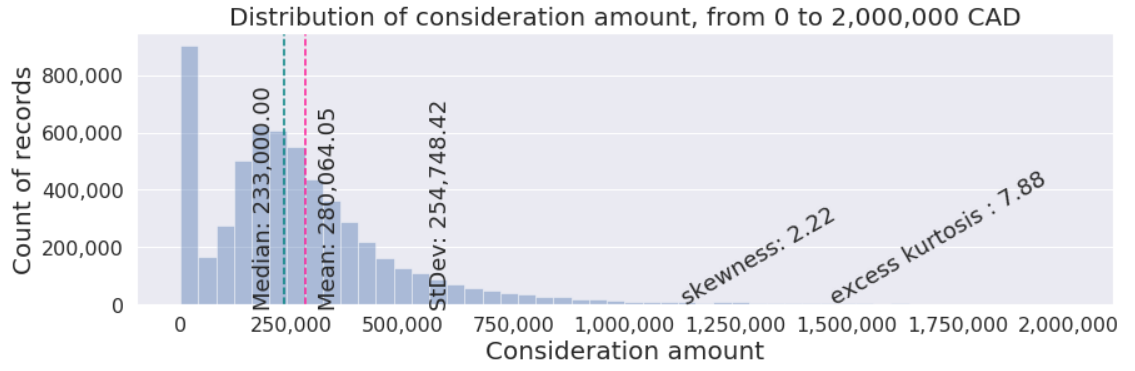
\includegraphics[width=.8\linewidth]{price_dist_raw.png}
        \caption{From 0 to 2'000'000 CAD}
    \end{subfigure}

    \begin{subfigure}{\linewidth}
        \centering
        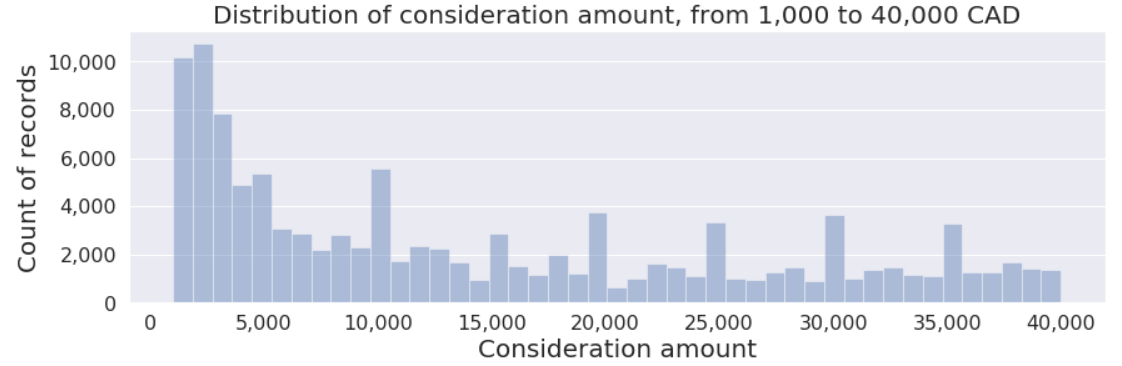
\includegraphics[width=.8\linewidth]{price_dist_zoom.png}
        \caption{From 0 to 40'000 CAD}
    \end{subfigure}
    \caption{Outliers at the bottom end of the price distribution most likely represent gift transactions.
    Large spike can be seen on the low end of the distribution.
    Since no clear break can be identified, 10'000 CAD was used as the cut-off threshold to filter Teranet records.}
    \label{fig:bottom_outliers}
\end{figure}

Since low outliers represent transactions that are not useful for analysis, they were removed from the dataset.
However, there is no way to establish what constitutes a reasonable bottom cut-off threshold, as there is no criteria available and there is no distinct break in the price distribution.
Since there seems to be en exceptionally large spike of transactions with consideration amount under 10'000 CAD, they were considered to be low outliers and were removed from Teranet's dataset, further reducing the number of records from 6,803,691 to 5,188,513.

In the case of outliers on the high end of the price distribution, they most likely correspond to transactions of expensive commercial and industrial property or whole residential buildings.
Since these transactions are useful for research questions concerning commercial and industrial property, they are left in the dataset and instead are marked with special features.
Since, again, there is no clear criteria for what would constitute an outlier, instead of using a single criterion, 7 different attributes are added that describe whether a record belongs to outliers according to a particular condition.
Examples of boxplots produced from two different criteria used to mark top outliers are presented on figure~\ref{fig:top_outliers}.

\begin{figure}[ht]
    \centering
    \begin{subfigure}{\linewidth}
        \centering
        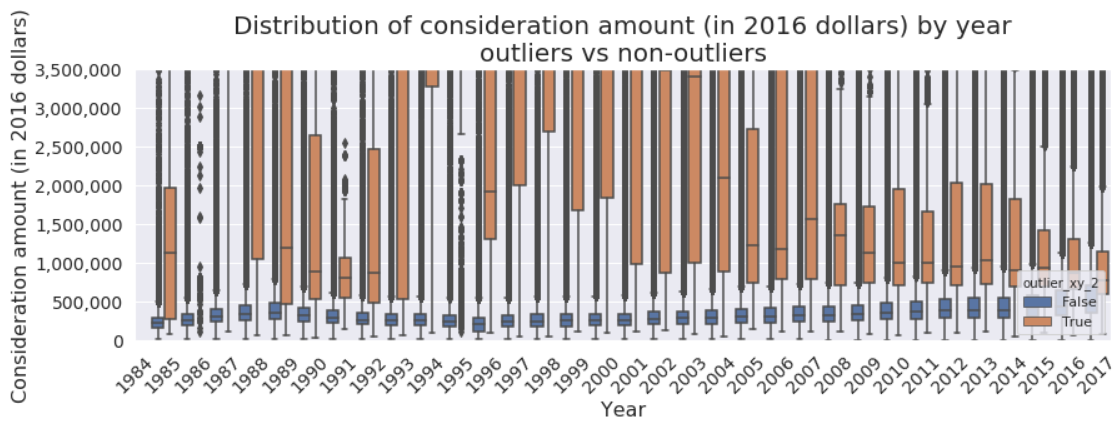
\includegraphics[width=.8\linewidth]{outliers_strict.png}
        \label{fig:top_outliers_mild}
        \caption{Outlier is 2 x median for 'xy'}
    \end{subfigure}

    \begin{subfigure}{\linewidth}
        \centering
        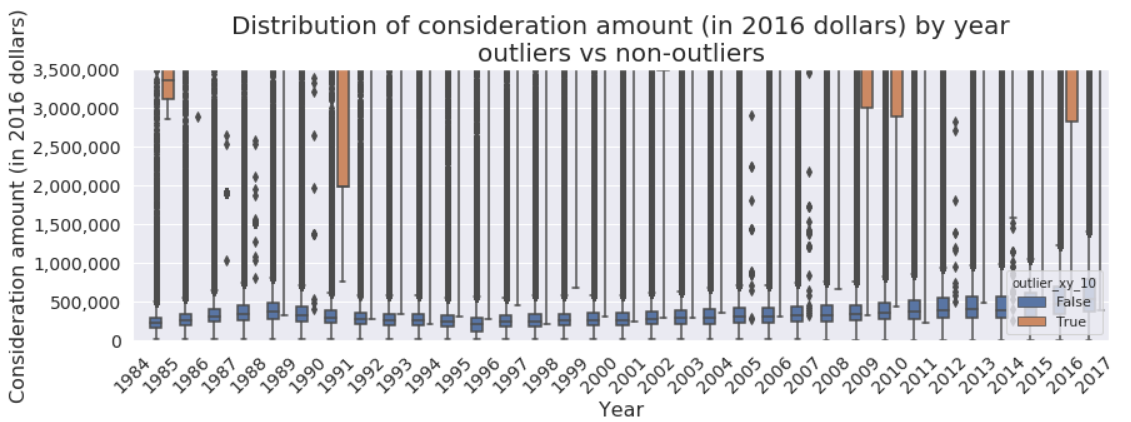
\includegraphics[width=.8\linewidth]{outliers_mild.png}
        \label{fig:top_outliers_strict}
        \caption{Outlier is 10 x median for 'xy'}
    \end{subfigure}
    \caption{Outliers at the high end of the price distribution most likely represent commercial, industrial and transactions of whole residential buildings.
    Since these transactions can still be useful for analysis, they are kept in the dataset and instead are marked using 7 new Boolean attributes representing criteria of varying strictness to define an outlier.
    The top subfigure presents an example where all transactions with price over 2 times greater than the median price for that 'xy' are considered to be an outlier, the bottom subfigure shows an example where only records with price over 10 times greater than median for 'xy' are marked as outliers.
    7 different criteria were used in total to mark top outliers.}
    \label{fig:top_outliers}
\end{figure}

For example, feature 'outlier\_y\_10' is a Boolean variable capturing if the price of a record, corrected for inflation, is over 10 times greater than the median price of all records for the corresponding year.
New attributes identifying outliers from the high end of the distribution in layers are added to each Teranet record and are used as features by the classification algorithm.

\section{Engineering new features for the classification algorithm} \label{sec:feature_engineering}

In addition to producing new keys for joining datasets, a number of new features is engineered from Teranet records to be tested with the classification algorithm (discussed in chapter~\ref{ch:ml_workflow}).
The new features are intended to give each Teranet transaction spatial and temporal "context" of the housing market dynamics by grouping Teranet records using various criteria.
For example, a feature 'xy\_prev\_sales' was added capturing the rolling count of Teranet records coming from this coordinate pair;
feature 'price\_to\_med\_year' captures a ratio of consideration amount of the current record to median consideration amount of all Teranet records for the corresponding year, etc.

The following features have been added to each Teranet record from 1985 to 2017 ('xy' represents 'x' and 'y' coordinates concatenated together as strings, used to group together all records coming from the same coordinate pairs):

\begin{itemize}
    \item 'price\_2016': consideration amount corrected for inflation using the coefficients from the Inflation Calculator provided by the Bank of Canada\cite{BankofCanada2019}
    \item 'pin\_total\_sales': count of Teranet records grouped by 'pin'
    \item 'xy\_total\_sales': count of Teranet records grouped by 'xy'
    \item 'pin\_prev\_sales': rolling count of Teranet records grouped by 'pin'
    \item 'xy\_prev\_sales': rolling count of Teranet records grouped by 'xy'
    \item 'xy\_first\_sale': a Boolean variable indicating whether it is the first record coming from this 'xy'
    \item 'pin\_years\_since\_last\_sale': difference in years since last record from this 'pin'
    \item 'xy\_years\_since\_last\_sale': difference in years since last record from this 'xy'
    \item 'xy\_years\_to\_next\_sale': difference in years to next record from this 'xy'
    \item 'da\_days/years\_since\_last\_sale': difference in days/years since last sale that occurred on this Dissemination Area
    \item 'xy\_sale\_next\_6m': a Boolean variable indicating whether there will be another sale on this 'xy' in the upcoming 6 month
    \item 'pin\_price\_cum\_sum': cumulative sum of inflation corrected price of all Teranet records from this 'pin'
    \item 'xy\_price\_cum\_sum': cumulative sum of inflation corrected price of all Teranet records from this 'xy'
    \item 'pin\_price\_pct\_change': percentage change of price corrected for inflation from the last Teranet record from this 'pin'
    \item 'xy\_price\_pct\_change': percentage change of price corrected for inflation from the last Teranet record from this 'xy'
    \item 'price\_da\_pct\_change': percentage change of price corrected for inflation from the last Teranet record from this Dissemination Area
    \item 'med\_price\_xy': median price corrected for inflation for all Teranet records from this 'xy'
    \item 'med\_price\_year': median price corrected for inflation for all Teranet records for this year
    \item 'price\_to\_med\_xy': ratio of price corrected for inflation to median price of all records for this 'xy'
    \item 'price\_to\_med\_year': ratio of price corrected for inflation to median price of all records for this year
    \item 'outlier\_y\_3': a Boolean variable marking as outliers all records with price more than 3 times greater than median for that year
    \item 'outlier\_y\_5': a Boolean variable marking as outliers all records with price more than 5 times greater than median for that year
    \item 'outlier\_y\_10': a Boolean variable marking as outliers all records with price more than 10 times greater than median for that year
    \item 'outlier\_y\_20': a Boolean variable marking as outliers all records with price more than 20 times greater than median for that year
    \item 'outlier\_xy\_2': a Boolean variable marking as outliers all records with price more than 2 times greater than median for that 'xy'
    \item 'outlier\_xy\_4': a Boolean variable marking as outliers all records with price more than 4 times greater than median for that 'xy'
    \item 'outlier\_xy\_10': a Boolean variable marking as outliers all records with price more than 10 times greater than median for that 'xy'
\end{itemize}

These new features were combined with TTS and Census variables via spatial and temporal relationships that were introduced in chapter~\ref{ch:spatial_and_temporal_relationships} and were used to train and test a classification algorithm to classify land use at Teranet transaction level, which will be described in chapter~\ref{ch:ml_workflow}.

\section{Chapter summary} \label{sec:data_preparation_summary}

The principles of ''Tidy data'', closely related to Codd's principles of database normalization, formalize the way how a shape of the data can be described and what goal should be pursued when formatting data.
The ''tidy data standard''  facilitates initial exploration and analysis of the data and simplifies the development of data analysis tools that work well together.
The structure of Teranet's dataset conforms with the ''Tidy data'' format.
Contrary to Teranet, tables with combined selected Census and TTS variables had variables for different Census and TTS years recorded as columns and thus needed to be ''melted''.
A new attribute 'year' was introduced to these tables to be used as a part of a composite foreign key when joining with Teranet records.

New foreign keys representing spatial identifiers, such as 'dauid' and 'taz\_o', were added to Teranet records via a series of spatial joins.
During the first join with Dissemination Area geometry used by Census, Teranet records with coordinates falling outside of GTHA have been filtered out.
Furthermore, Teranet records with consideration amount under 10'000 CAD were considered to be outliers at the low end of price distribution and were removed from the dataset.
Outliers at the high end of the price distribution were not removed, but instead were marked through 7 new Boolean attributes using various criteria to define a top outlier.
Finally, new features have been engineered to be tested with classification algorithms in chapter~\ref{ch:ml_workflow}.

\vspace{5mm}

Characteristics of the raw Teranet dataset:
\begin{itemize}
    \item 9,039,241 rows
    \item 15 columns
\end{itemize}

Characteristics of the Teranet dataset after data preparation described in this chapter:
\begin{itemize}
    \item 5,188,513 rows
    \item 75 columns
\end{itemize}

\chapter{Database design for GTHA housing market data} \label{ch:database_design_for_gtha_housing_market_data}

\section{Intro: databases} \label{sec:intro_database_design}

%TODO write chapter introduction
Something about Knowledge Discovery in Databases

\section{Requirements to the information system for housing market data} \label{sec:requirements_to_information_system}

%TODO check requirements
On one hand, for such information-handling system to be comprehensive, it needs to combine a wide range of data sources describing these systems while maintaining semantic interoperability between these sources.
In the case of land use, transportation, demographic, and real estate data, it means to take into account the varying spatial and temporal scale and resolution between these data sources when joining them together.
At the same time, the system needs to be easily accessible to a wide range of researchers and students;
it also needs to have powerful data processing capacity, to allow working with and performing calculations on large datasets related to real estate and land use.
In addition to that, the system should have a modular structure, have a workflow that is reproducible and modifiable, so that new data sources and new relationships can be added to the system, while maintaining the existing part intact.

All of the requirements listed above present a strong case for the housing market information system to be implemented in a form of a relational database.
Given the size of the datasets and the current research needs, PostgreSQL presents a good option for the database management system that fits all the discussed criteria.
The focus of this master thesis is the organization and implementation of the GTHA housing market database to facilitate future research activities focused on the Longitudinal Analysis of housing sales in the Greater Toronto-Hamilton Area conducted by the University of Toronto Transportation Research Institute (UTTRI).

\section{Philosophy of the housing market database} \label{sec:housing_market_database_philosophy}

%TODO describe the philosophy behind attribute-based spatial and temporal joins
attribute-based database defined by spatial relationships

\section{Entity relationship diagrams of GTHA housing market database} \label{sec:entity_relationship_diagrams_in_gtha_database}

%TODO include ER diagrams for the database

\section{Attribute and referential integrity constraints} \label{sec:constraints_database}

\subsection{Primary keys used in the database} \label{subsec:primary_keys_in_gtha_database}

%TODO write about primary keys in the database

\subsection{Referential integrity constraints used in the database} \label{subsec:referential_integrity_constraints_in_gtha_database}

%TODO write about referential integrity constraints in the database

\section{Chapter summary} \label{sec:rdbms_design_summary}

All the requirements have been met via appropriate constraints.
%TODO write chapter summary

\chapter{Results of the Exploratory Data Analysis (EDA)} \label{ch:eda_results}

\section{Intro: Exploratory Data Analysis (EDA) of Teranet dataset} \label{sec:eda}

%TODO write chapter introduction
something about the philosophy of EDA,
something about ESDA
what has been done with Teranet data

\section{Results of EDA of Teranet dataset} \label{sec:eda_results_teranet}

%TODO write a section about EDA results for Teranet

\section{Results of ESDA of Teranet dataset} \label{sec:esda_results_teranet}

%TODO write a section about ESDA results for Teranet

\section{Chapter summary} \label{sec:eda_summary}
EDA and ESDA explore some basic characteristics and establish some code to look at this data.
%TODO write chapter summary

\chapter{Conculsion} \label{ch:conclusion}

Microsimulation models present the latest generation of integrated land use and transportation models and are well suited to analyze the complex interaction of transportation and land use.
New data sources that appear with the increased digitization of human activity present opportunities to look at urban processes at unprecedented spatial and temporal scale, and thus present a lot of value for design and validation of integrated urban models and for longitudinal studies concerned with evolution of urban form.
Introduction of POLARIS electronic land registration system by the Province of Ontario in 1985 lead to the creation of an extensive dataset of real estate transactions by Teranet Enterprises Inc.
However, despite having very high spatial and temporal resolution, available version of Teranet's dataset suffered from severe lack of features describing each individual transaction.

One of the major attributes missing from Teranet data is the type of property being transacted, or land use information for the parcel where a transaction is recorded.
Along with selected Census and TTS variables, detailed parcel-level land use from the Department of Geography and DMTI land use data have been spatially joined to each Teranet record.
However, since both of these data sources have their limitations, detailed land use data from Department of Geography has been used to train an algorithm capable of classifying land use based on the housing market dynamics;
this way, land use information can be made available for each Teranet record for the full timespan covered by the Longitudinal Housing Market Research conducted by UTTRI .

To augment Teranet's dataset, new variables were engineered from its native attributes to capture the housing market dynamics at the parcel level:
for example, 'xy\_total\_sales' was computed as the total count of Teranet records coming from a particular coordinate pair;
'med\_price\_xy' represents the median price of all records coming from a coordinate pair, etc.
To augment Teranet data with demographic and transport information, the new Teranet features were spatially and temporally joined with Census and TTS variables recorded at the level of a Dissemination Area and TAZ zone, respectively.
Finally, the augmented Teranet dataset has been tested with machine learning algorithms, attempting to classify land use for each Teranet record within the span of Census / TTS variables, thus recognizing land use changes with time.

A range of preprocessing techniques has been tested with several linear, tree-based and nearest neighbors classification algorithms;
tree-based models and $k$-Nearest Neighbors significantly outperformed linear models.
The new features engineered from native Teranet attributes have shown to have strong predictive power when classifying land use.
When joined with Census variables at the level of Dissemination Areas, new features engineered from Teranet's dataset allowed the classification of land use with a high level of accuracy.
Random Forest model was trained using random 70\% sample of all Teranet records with new features from 2011 to 2014 stratified by target classes (''condo'', ''house'', or ''other'');
the model achieved 97\% of accuracy on the test subset composed of the remaining 30\% of records from 2011 and 2014.
Tree-based models did show some degree of overfitting and could benefit from further increase in the size of training data, as indicated by their learning and validation curves.

Features engineered from native Teranet attributes that capture price ratios to median and frequency of transactions from a coordinate pair have strong predictive power for land use classes, as indicated by feature selection techniques and model coefficients.
This workflow could be further improved by joining more Census / TTS variables to engineer new features;
target classes also could be redefined to allow more meaningful classification.
In addition, results of the classification preformed by this workflow need to be investigated.
A map produced with counts of misclassified Teranet records per DA shows that errors seem to be highly concentrated and correspond to high-frequency transactions, such as condos and mixed use properties.
To facilitate further investigation of classification results, augmented Teranet dataset with new feature 'lucr\_predict' along with related Census and TTS tables has been transformed into PostgreSQL relational database to facilitate ease of access by a broader group of specialists.
Entity Relationship (ER) diagram for the database created as a part of this master's thesis can be found in Appendix~\ref{ch:appendix_rdbms};
its referential integrity constraints were implemented based on the spatial and temporal relationships between data sources that were introduced in chapter~\ref{ch:spatial_and_temporal_relationships}.


%% This adds a line for the Bibliography in the Table of Contents.
\addcontentsline{toc}{chapter}{Bibliography}
%% *** Set the bibliography style. ***
%% (change according to your preference/requirements)
\bibliographystyle{plain}
%% *** Set the bibliography file. ***
%% ("thesis.bib" by default; change as needed)
\bibliography{thesis}

%% *** NOTE ***
%% If you don't use bibliography files, comment out the previous line
%% and use \begin{thebibliography}...\end{thebibliography}.  (In that
%% case, you should probably put the bibliography in a separate file and
%% `\include' or `\input' it here).

\end{document}
